\thispagestyle{empty}%
\begin{tikzpicture}[remember picture, overlay]
  % Background Julia Set
  \node[inner sep=0pt] at (current page.center) {%
    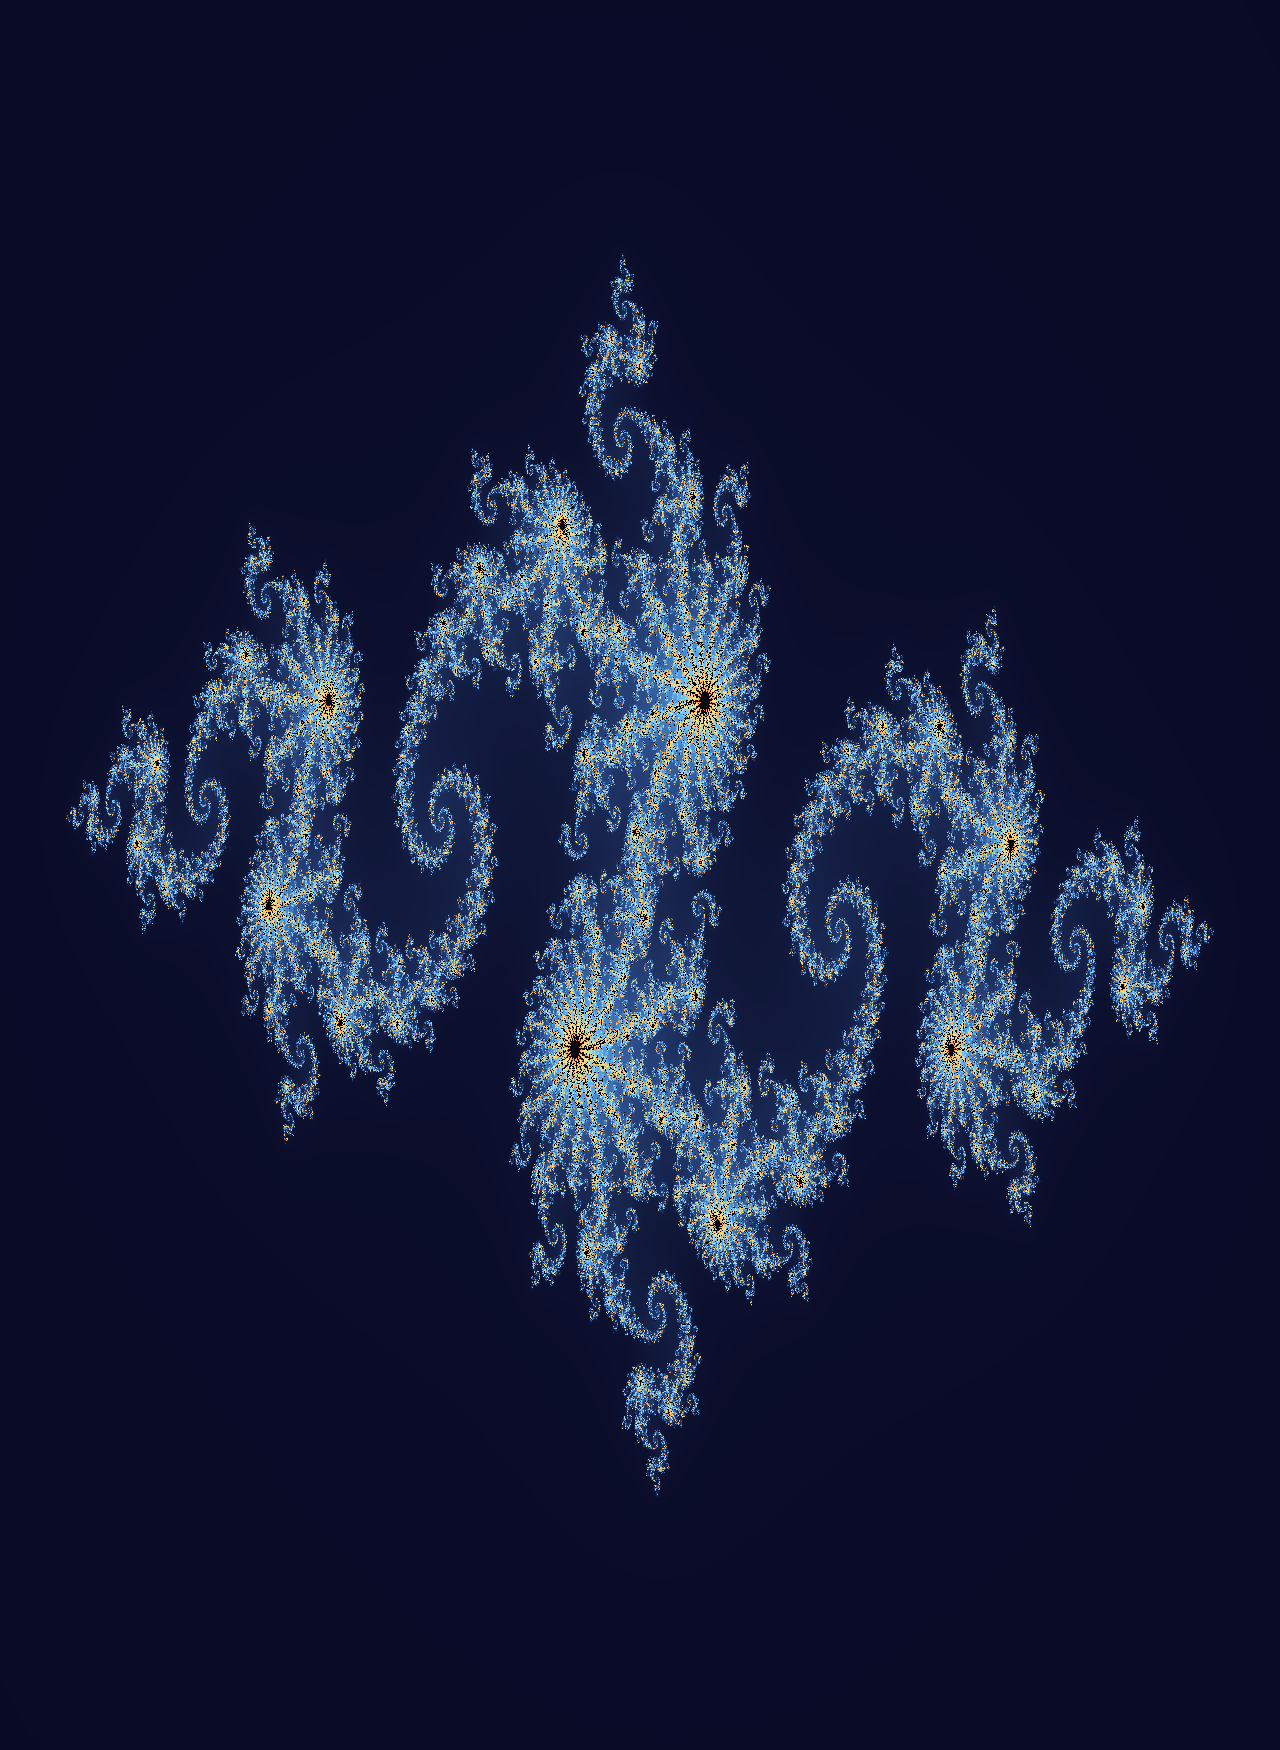
\includegraphics[width=\paperwidth,height=\paperheight]{assets/julia-matte-bg.png}%
  };
  % Dark overlay for text readability
  \fill[black, opacity=0.4] (current page.south west) rectangle (current page.north east);
  
  % Foreground Text
  \node[anchor=center, text=white] at (current page.center) {%
    \begin{minipage}{0.92\textwidth}
      \centering
      \bfseries
      {\fontsize{26}{32}\selectfont HSC Mathematics Extension 2\par}%
      \vspace{0.55cm}%
      {\fontsize{36}{44}\selectfont Collection of Hard Problems\par}%
      \vspace{0.55cm}%
      \noindent\raggedleft{\large Vu Hung Nguyen\par}%
    \end{minipage}%
  };
\end{tikzpicture}%
\clearpage
